\documentclass{ltjbook}
\usepackage{docmute} 
\usepackage{../../myStyle} 

\begin{document}
\VerbatimFootnotes
\chapter{Regression analysis using R}
\label{m11_MRonR}

So far, we have explained in words the mechanisms of regression analysis and \keytermE{multiple regression analysis}. However, it's all in vain if you can't calculate the results yourself. We haven't explained the method of calculating the regression coefficients for multiple regression analysis, but when calculating with R, it can be expressed without distinguishing between simple regression and multiple regression. Let's learn how to do it all at once here.

\section{Reconfirming the R environment}
We have explained how to use R in Chapters \ref{m03_introR} and \ref{m04_usingR}. Let's proceed while reviewing them.

\subsection{Preparation of Environment (Verification)}
First, let's prepare the environment. We assume that R and RStudio have already been installed\footnote{If you haven't installed them yet, please go back to Chapter \ref{m03_introR} and catch up. You can search for "RStudio installation" online, and you'll find many sites with helpful guidance.}. The following text will be based on this assumption.

Please follow these three steps to prepare for the execution.
\paragraph{Starting RStudio}Please start RStudio. Note that in some cases, such as when installing packages, you may need administrative privileges. If you are using Windows, it may be a good idea to run as an administrator.
\paragraph{Opening a project} It is fine to use the project created the last time. Let's create a new script file in the same folder as last time. Select "Open Project" from the menu (File $\to$ Open Project), and choose the \texttt{.Rproj} file in the desired folder. This file contains information about the project, and selecting it will set the working directory to the corresponding folder. You can confirm whether the project has been opened by checking the upper right corner or menu bar in RStudio.
\paragraph{Opening an R script} Let's prepare an R script file to write today's code. Go to File > New File > R Script and open a blank R script file. Once you have opened the blank file, you can proceed to write your code. You can also continue writing in the Rmd file if that is more convenient.

You are now prepared to write code in the script section.

There should be a lot of data related to statistics to the point where it becomes too much to manually input. This time, we will also read the data from a file to use. When reading from a file, it's important to pay attention to the text encoding. If the encoding is different, it may result in garbled characters when reading ASCII data\footnote{If you're not sure what this means, please refer to Appendix \ref{computer}.}. For people using Windows with the non-standard encoding Shift-JIS (CP-932), they may need to specify the world-standard UTF-8 when reading.

This time, let's load the data of the same baseball players as in the exercise of Chapter \ref{m04_usingR}. Please run the following three lines.

\begin{lstlisting}[language=c++,label={code:11_01},caption={環境の初期化とパッケージ，ファイルの読み込み}]
rm(list=ls())
library(tidyverse)
dat <- read_csv("baseballDecade.csv", na="NA", 
        locale=locale(encoding="utf8")) %>% 
        filter(Year=="2020年度")
summary(dat)
\end{lstlisting}


\paragraph{Code Explanation}
\begin{description}
   \item[1行目] 環境Environmentを初期化するコードです。Rmd形式で書いている人はこの行は書かないようにしてください\footnote{Rmdファイルはそのまま使うのではなく，出力ファイル形式に\verb|knit|して使います。 その際必ず環境情報は初期化されるので書く必要がなく，むしろ書いてあると \verb|knit| するファイルの情報なども消してしまうので \verb|knit| できなくなるのです。}\footnote{Rmdで保存するときの拡張子は\verb|.Rmd|になります。ファイル名にピリオドが入っていると拡張子が変わっちゃうことがあるので，注意してください。拡張子って何，というひとは\ref{suffix},Pp.\pageref{suffix}を参照。}。
   \item[2行目] \texttt{tidyverse}パッケージを読み込んでいます。このパッケージはファイルの読み込みや並べ替え操作など，便利な機能がまとめられたものです。
   \item[3-4行目] \texttt{baseballDecade.csv}というファイルを読み込んでいます。このファイルがプロジェクトフォルダ内にあることを確認してから実行してください。
   \item[5行目] ファイルの一部，2020年度のデータだけに絞るようフィルターをかけています。
   \item[6行目] 読み込んだデータの記述統計量など，基本的な要約を行っています。
\end{description}


\subsection{Drawing Scatter Plots}
When you have data, the first thing to do is visualize it. Don't forget the promise to \textbf{make data into a figure}.
There are various variables in this case, but I would like to extract only the data of the batter's height and weight and create a figure.

\begin{lstlisting}[language=c++,label={code:11_02},caption={Initialization of the environment, installation of packages, and reading of files}]
batter <- dat %>%
  dplyr::filter(position != "pitcher") %>%
  dplyr::select(height, weight)
g <- ggplot(batter, aes(x = height, y = weight))
g <-  g + geom_point()
g
\end{lstlisting}

\paragraph{Code Explanation}
\begin{description}
   \item[1-3 lines] Creating an object named \texttt{batter}. This is done by processing the \texttt{dat} object, which will be explained later in detail.
   \item[4th line] Using the \texttt{batter} object, specify the x-axis as the \texttt{height} variable, and the y-axis as the \texttt{weight} variable on the canvas.
   \item[5th line] Plotting points on the canvas using \verb|geom_point|.
   \item[6th line] Displaying the plotting object named \texttt{g}.
\end{description}


As long as the resulting figure looks like Figure \ref{fig::11_01}, it is OK.

\begin{figure}[ht]
   \centering
   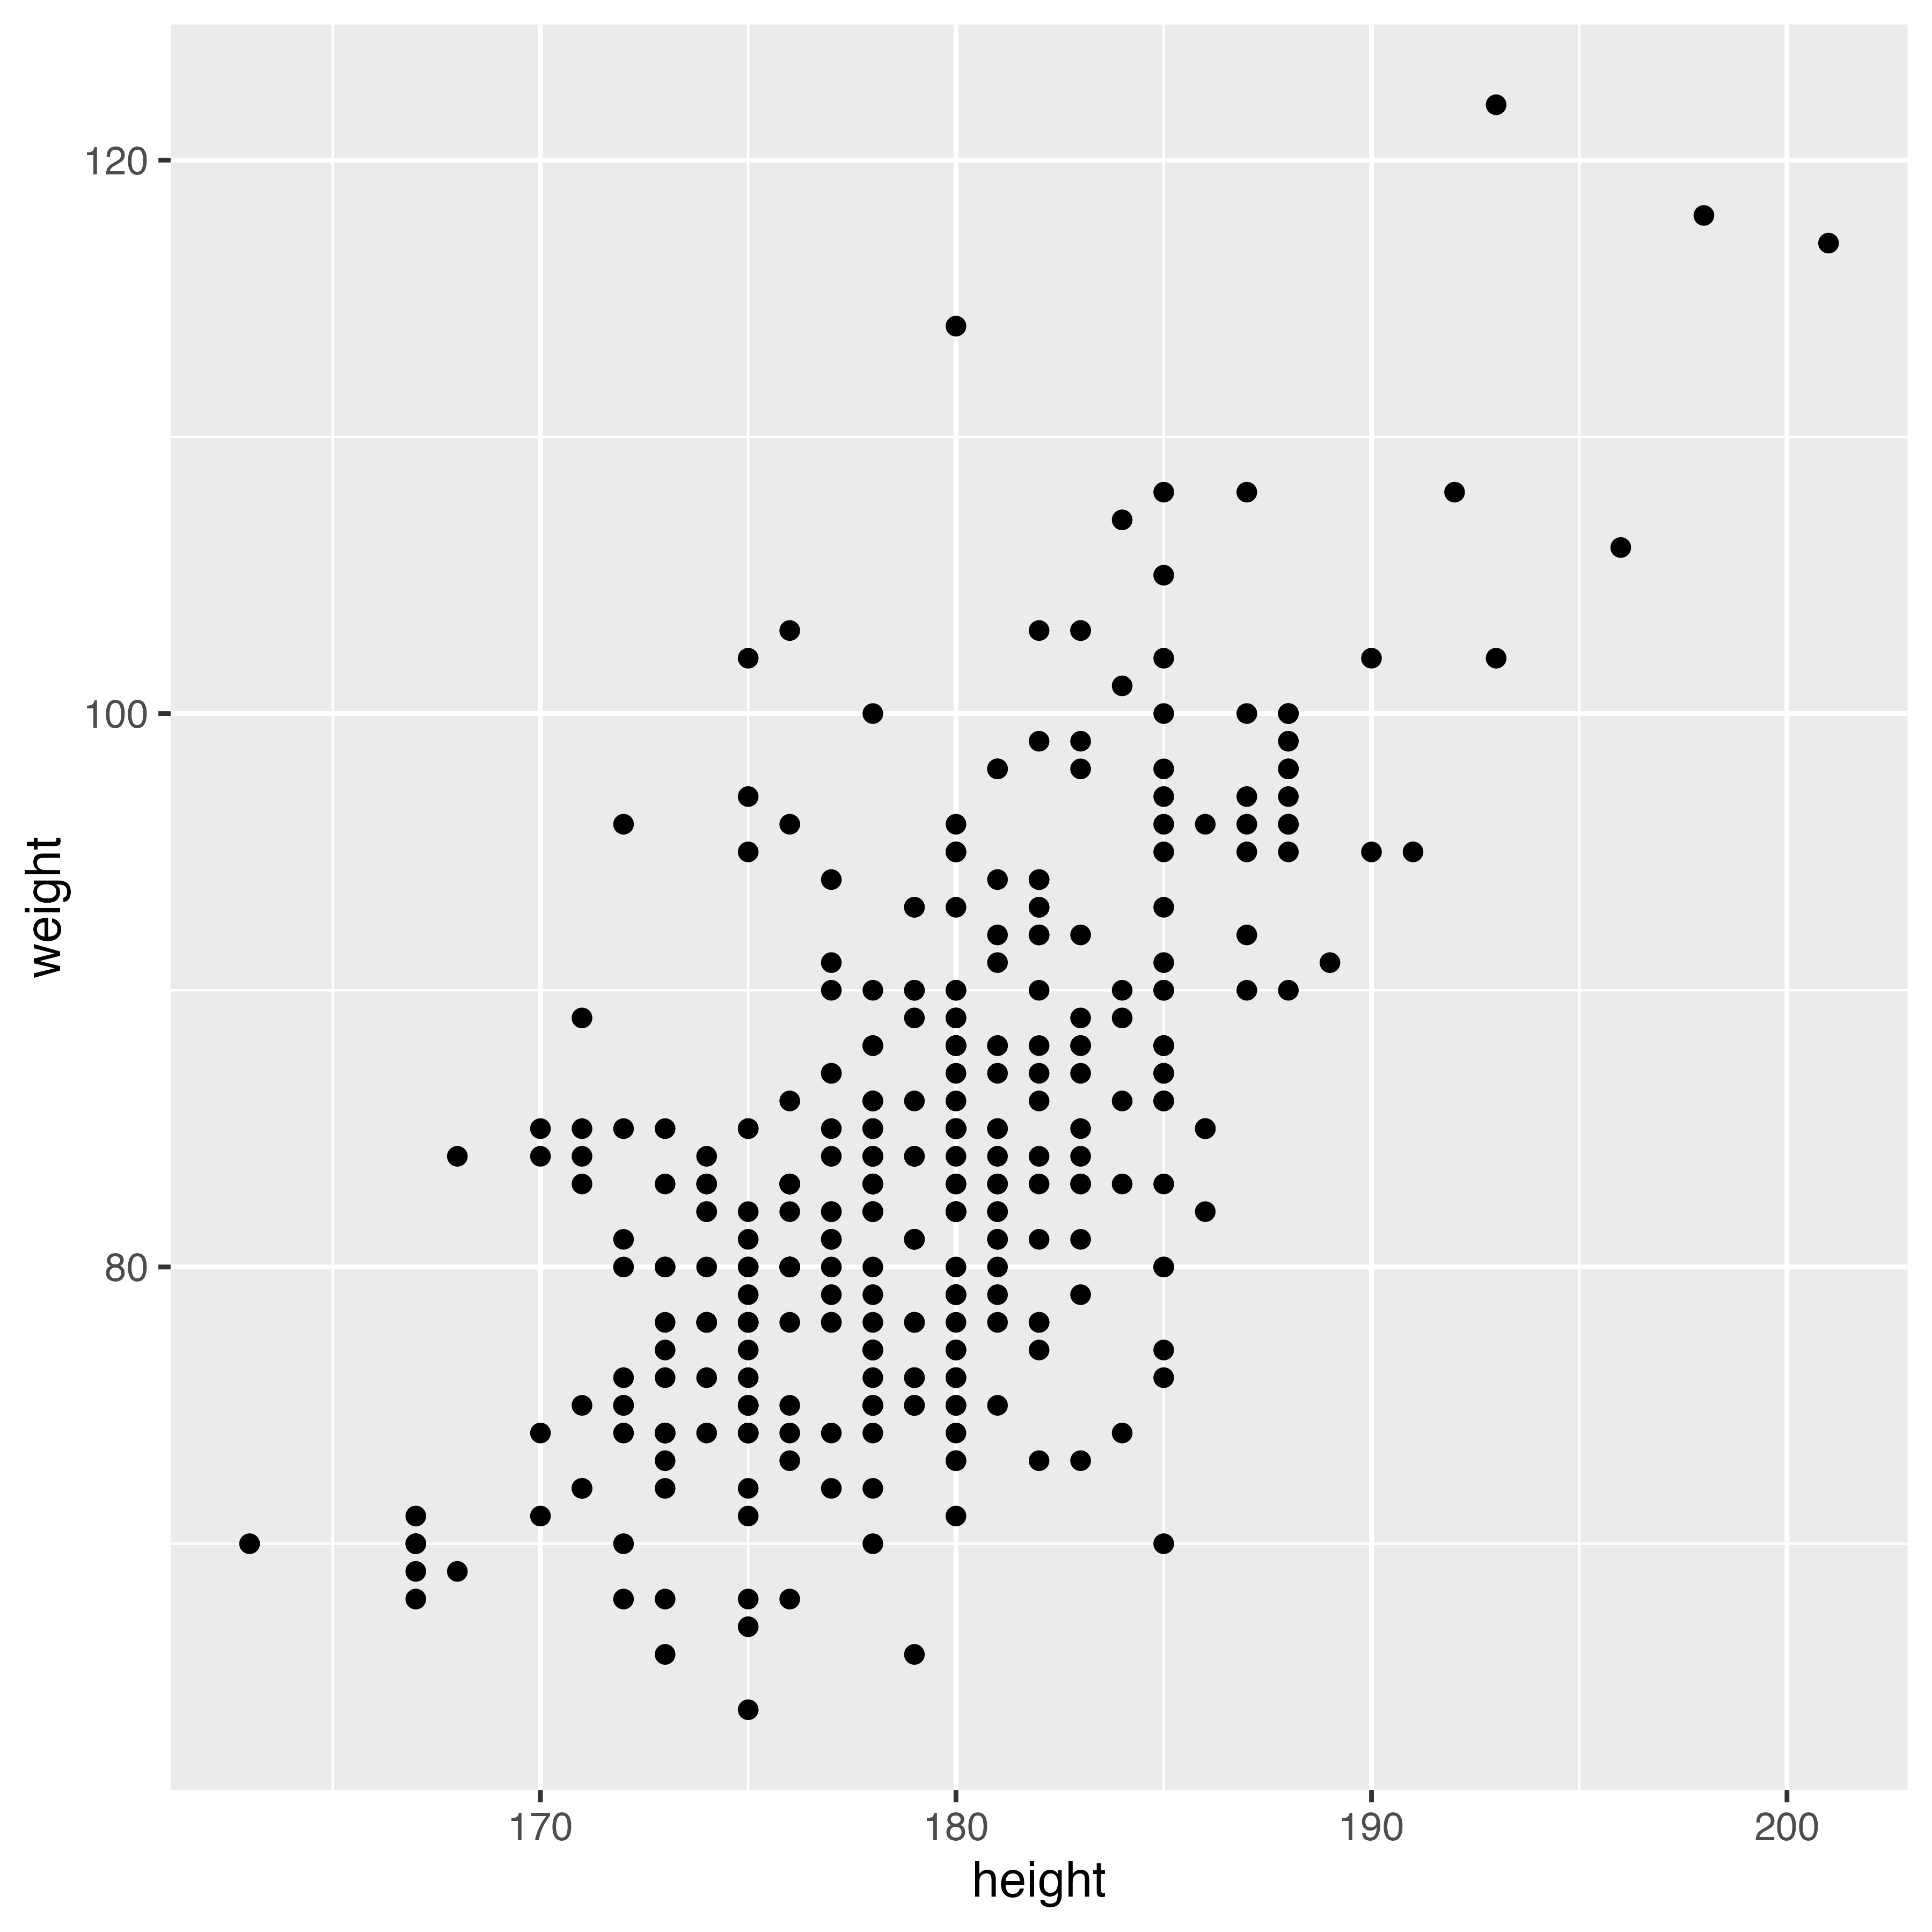
\includegraphics[keepaspectratio,width=0.65\linewidth]{../images/11_MultipleRegressionOnR/Rplot11_01.png}
   \caption{Data for height and weight}
   \label{fig::11_01}
\end{figure}


Regarding the operations in lines 1-3, what I wanted to do here was to extract the variables for height and weight from the "dat" object, but only for data related to batters. Please note that the TeX code should not be modified.
These operations are implemented using the \texttt{filter} function and the \texttt{select} function in the \texttt{dplyr} package, which is included in the \texttt{tidyverse} package. For more information on the difference between these two functions, please refer to Section \ref{dataHandling}, Pp. \pageref{dataHandling}.
Anyway, with this, a scatter plot of the desired data can be created, and it appears that there is a positive correlation.
It seems okay to assume a linear relationship. By the way, you can draw a straight line with \texttt{ggplot} by writing the following code.

\begin{lstlisting}[language=c++,label={code:11_03},caption={回帰線を引く}]
g <- g + geom_smooth(method = "lm", se = FALSE)
g
\end{lstlisting}

\paragraph{Code Explanation}
\begin{description}
   \item[Line 1] A smoothing function \verb|geom_smooth| is used on the object \texttt{g}, which draws a smooth line on the data. The line is drawn using \keytermE{linear model}{せんけいもでる} (\texttt{lm}).
   \item[Line 2] The object \texttt{g} is plotted.
\end{description}


\section{Executing Linear Regression}
Let's now perform regression analysis. Regression analysis is called a linear model because it fits a linear function. The \texttt{lm} function, which stands for the initials of this, is a linear regression model. Let's try running the following code (\texttt{code:\ref{code:11_04}}).
\begin{lstlisting}[language=c++,label={code:11_04},caption={Executing Regression Analysis}]
    result <- lm(weight ~ height, data= batter)
    summary(result)
\end{lstlisting}


\paragraph{Code Explanation}
\begin{description}
   \item[1行目] \texttt{lm}関数に回帰式とデータを入れて分析を実行し，その結果を\texttt{result}オブジェクトに代入する。ちなみに\verb|~|はチルダといいます\footnote{日本語キー配列の場合，「ほ」の右，アットマークの上にある「へ」のキーをShiftを押しながら押すと出ます。USキー配列の場合はtabキーの上にあります。}。
   \item[2行目] 分析結果の要約を出力させる。
\end{description}


What's important here is the expression of the regression equation in the first line. In R, $y\sim x$ represents $y=f(x)$, which expresses the relationship between the dependent variable $y$ and the independent variable $x$. This notation, called \keytermE{formula}, is used not only for regression equations but for expressing the relationship between dependent and independent variables with the $\sim$ sign. Although the expression used here used the function \texttt{lm}, when expressing the relationship between independent and dependent variables with non-linear models, it is still represented as \verb|y ~ x|. Getting used to this notation makes it easy to understand that both this analysis and that analysis are simply $y=f(x)$ in form. This time, it represents predicting weight using height.

The output results of this analysis are shown in Output \ref{RS:out11_01}.

\input{m11_Regression_onR_escape_10}

There seems to be various things going on, but let's check them one by one. First, we have the word \texttt{Residuals}, which represents the descriptive statistics of the residuals $e_i$. It would be good to check how large the residuals can be.
The term "Coefficientes" refers to coefficients. Here we have regression coefficients. It may be a little difficult to read, but it is in tabular form, and the section labeled "Estimate" represents the estimated value, which is the value we are interested in finding for the regression coefficient. The TeX code will not be modified.
The regression equation is as follows.

\[ \hat{y} = -124.91755 + 1.16670 \times height \]

Please make sure to confirm which number corresponds to what result. Also, by obtaining this equation, you can understand that by inputting a new number for height, it is possible to predict weight.

There is also various other information available, but it pertains to inferential statistics that will be discussed in the latter part of the course, so it's okay if you don't know it yet. To briefly explain, an estimated value is not a value obtained from the data used in this study. Instead, it means that when considering this data as a sample taken from a larger population, the value obtained from this sample can be used to make inferences about the relationship in the population. You may think that instead of estimating from the sample, we can consider the characteristics of the sample to obtain the answer using the least squares method, but I'm not explaining that now. Luckily, the value obtained using the maximum likelihood method, which is used here, and the regression coefficients obtained using the least squares method match. Also, we calculate the potential difference in estimated values when using a different sample other than the one used in this study, which is depicted in the "Std.Error" part. Accordingly, we examine the likelihood of the regression coefficient being 0, indicating that the explanatory variable isn't predictive, and derive conclusions from the "t value" and "Pr(>|t|)" parts while considering what can be inferred from this analysis.
More important than that is the line below, which says \texttt{Multiple R-squared}. This is the so-called $R^2$ value and indicates how well the model fits the data. In this case, $R^2=0.4096$, which means that the correlation coefficient between the predicted values $\hat{y}$ and the dependent variable $y$ is about 0.62, and the proportion of variance explained is about 40.9\%. As for the goodness-of-fit, it can be said to be somewhat poor.

\section{What we can learn from residuals}
Inside the object that stores the results returned by the \texttt{lm} function in this case, there is other information such as the predicted values $\hat{y_i}$ and the residuals $e_i$. To confirm that these are not fictional values but calculated values, let's display them.

\begin{lstlisting}[language=c++,label={code:11_05},caption={Other information on regression analysis}]
batter <- batter %>% 
    dplyr::mutate(residuals = result$residuals,
                    yhat = result$fitted.values) 
batter
summary(batter)
plot(batter)
cor(batter)
\end{lstlisting}


\paragraph{Code Explanation}
\begin{description}
   \item[1-3 lines] Overwrite the \verb|batter| object with a modified version of the \verb|batter| object. The modification is done using the \verb|mutate| function from the \verb|dplyr| package to add variables. The added variable names are \verb|residuals| and \verb|yhat|. For \verb|residuals|, the \verb|residuals| variable from the \verb|result| object is assigned, and for \verb|yhat|, the \verb|fitted.values| variable from the \verb|result| object is assigned.
   \item[4th line] Display the overwritten \verb|batter| object. Only the top portion is displayed as it is very long.
   \item[5th line] Display summary statistics of the overwritten \verb|batter| object.
   \item[6th line] Draw a plot of the \verb|batter| object.
   \item[7th line] Calculate the correlation coefficient of the \verb|batter| object. 
\end{description}


The object "result", which contains the results of the regression analysis, includes the residuals as a variable called "residuals". It also includes predicted values as a variable called "fitted.values". Let's take a look at a part of the output from the fourth line (Output \ref{RS:out11_02}).
\begin{Rscreen}{Output results of Regression Analysis}{out11_02}
   \begin{verbatim}
# A tibble: 329 × 4
   height weight residuals  yhat
    <dbl>  <dbl>     <dbl> <dbl>
 1    171     72   -2.59    74.6
 2    181     98   11.7     86.3
 3    177     91    9.41    81.6
 4    180     85   -0.0882  85.1
 5    171     84    9.41    74.6
\end{verbatim}
\end{Rscreen}


When looking at this, for example, the data on the first line is for a player who is 171cm tall and weighs 72kg, and the calculation using the regression equation of $-124.91755+1.16670\times height$ shows a resulting value of 74.6. The predicted value $\hat{y_1}$ of 74.6 differs from the actual value $y_1$ by 2.59, so the difference $\hat{y_1}-y_1$ is -2.59. Similarly, predictions and residuals could be calculated for each of the 329 data points.

Let's take a look at the plot again. This is not an output using \texttt{ggplot}, but rather an example of the original R output (which is why it's a bit less visually appealing), but you may notice a few things when looking at it.
One of the places where the combination of \verb|height| and \verb|yhat| is linear. The next \verb|cor| function also shows a corresponding value of 1.0. This is natural because the predicted value is the height data stretched and shifted, so these two are one-to-one correspondence, with a correlation of 100%. Additionally, the combination of the explanatory variable \verb|height| and the residuals \verb|residuals| is closer to a circle, and the correlation coefficient is almost 0.0\footnote{Wait a minute; it seems like there is some number shown somewhere. You might notice the display of $5.451636e-16$ in the calculation results. This expression means that the value is too large to be expressed in normal decimal notation, and the part "e+" represents a power of 10. In this case, it's "e-16", so the value $10^{-16}=0.00000000000000001$ is multiplied by 5.451636, giving us the answer. Although it can be mathematically proven to be exactly 0.0, machine calculations have round-off errors, resulting in a slight deviation. However, it is effectively zero.}. It's fundamentally odd to have a correlation between the explanatory variable and the residuals. The explanatory variable tries to explain the dependent variable as much as possible, and the remainder is the residuals. Therefore, if there is an element related to the explanatory variable in the residuals, it means that it is still an explainable part of the dependent variable, not the residuals.

Similarly, the correlation between the residuals and predicted values, \verb|residuals| and \verb|yhat|, is also almost 0.0. This is theoretically supposed to be $0.0$, as regression analysis separates the explained part (predicted values) and the unexplained part (residuals) precisely based on the explanatory variables, so there should be no relationship left between the separated parts. Although the mathematical derivation can be found in \citet{kosugi2018}, pages 127--135, it should be obvious by looking at the data.
\section{Multiple Regression Analysis}
Next, let's move on to \keytermE{multiple regression analysis}{じゅうかいきぶんせき}. Performing multiple regression analysis in R is a simple task, as you only need to add one explanatory variable. However, it is important to remember that careful interpretation of the results is necessary. Note that the TeX code will not be modified.

\begin{lstlisting}[language=c++,label={code:11_06},caption={Creating and visualizing data for multiple regression analysis}]
batter2 <- dat %>%
    dplyr::filter(position != "Pitcher") %>%
    dplyr::select(HR, Hit, salary) %>%
    na.omit()
g1 <- ggplot(batter2, aes(x = HR, y = salary)) +
    geom_point()
g1
g2 <- ggplot(batter2, aes(x = Hit, y = salary)) +
    geom_point()
g2
cor(batter2)
\end{lstlisting}


\paragraph{Code Explanation}
\begin{description}
   \item[1-4th line] Creating an object named \texttt{batter2}. This is made by processing the \texttt{dat} object. In the 2nd line, selecting fielders (non-pitchers), and in the 3rd line, selecting home runs, hits, and salary as variables. The 4th line removes missing values all at once, because players who have not hit any home runs cannot be included in the data.
   \item[5-7th line] A scatter plot with the number of home runs on the x-axis, and salary on the y-axis is drawn.
   \item[8-10th line] A scatter plot with the number of hits on the x-axis, and salary on the y-axis is drawn.
   \item[11th line] Examining the correlation of the data with numbers.
\end{description}


Looking at the plot, it seems like the more home runs and hits a player gets, the higher their salary is (see Figure \ref{fig::11_03}). It's no wonder that professional baseball is a world where skill determines success, and where there's money to be made on the field. There are a lot of players on the left side of the data who don't hit many home runs or make many hits, so there's a possibility that the high correlation coefficient is being influenced by the strong performers. Additionally, there seems to be a correlation between hits and home runs which is a bit concerning. However, for now let's proceed with our analysis using this dataset.

\begin{figure}[ht]
	\centering
	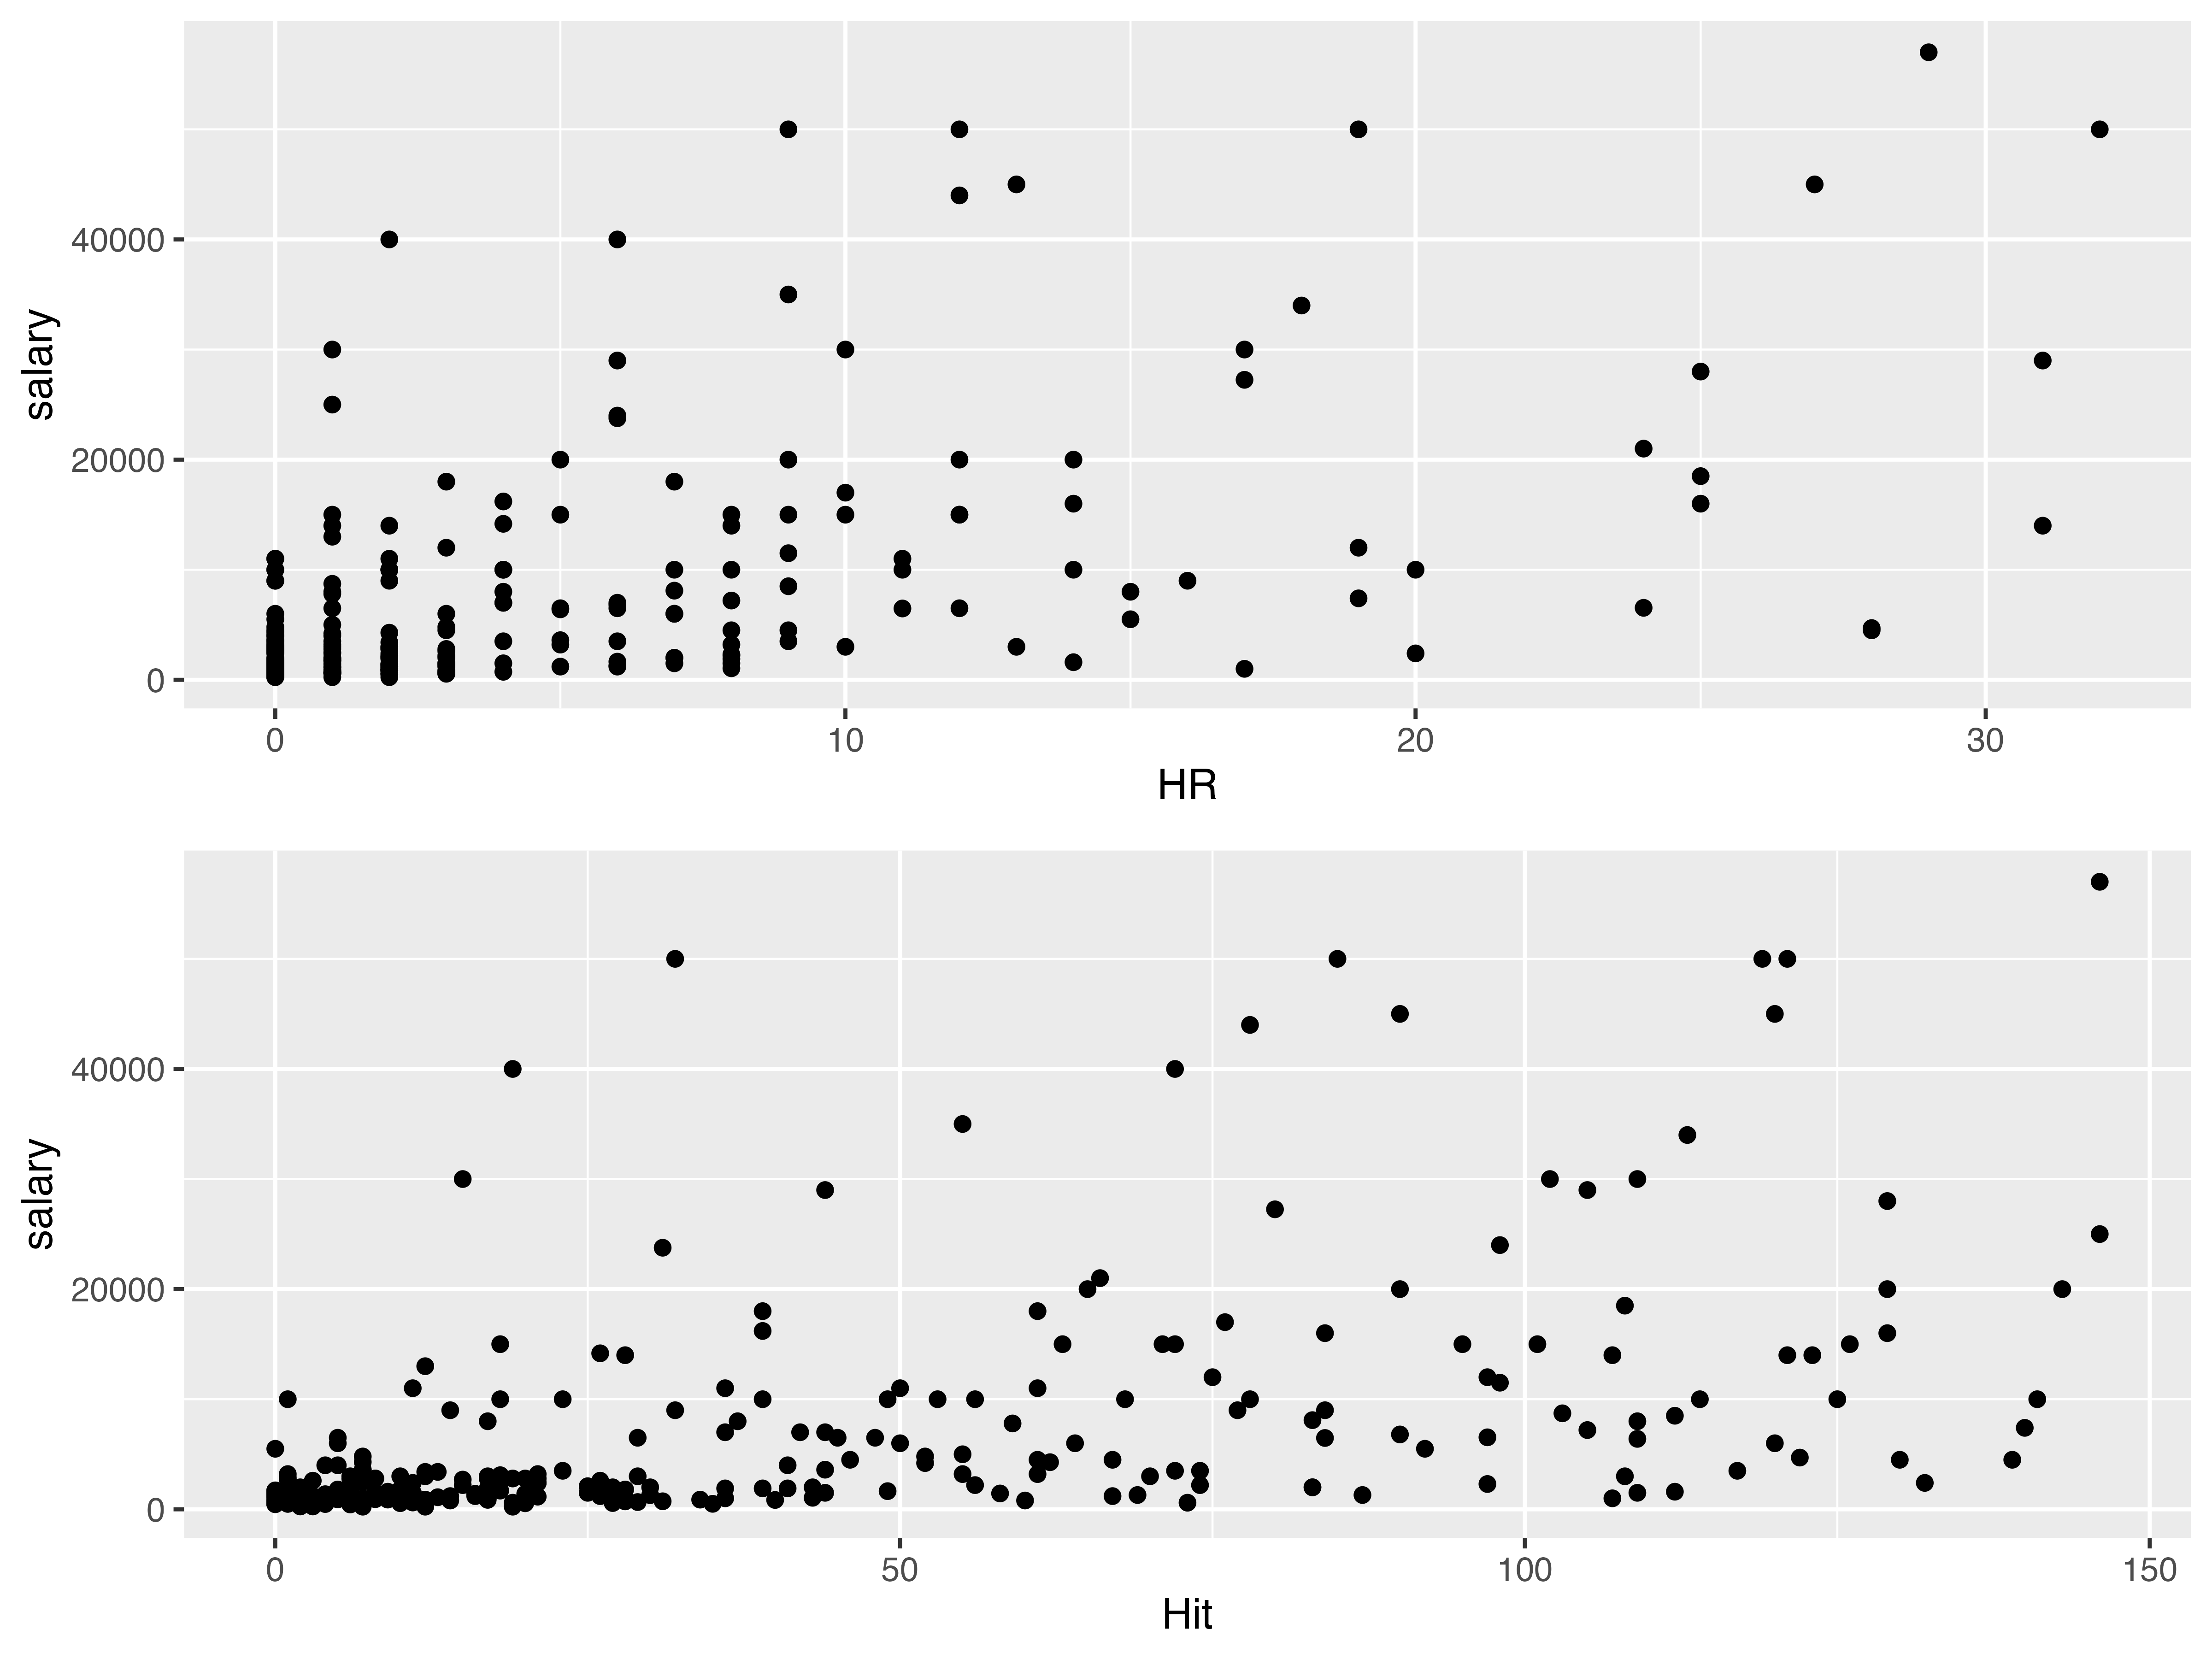
\includegraphics[keepaspectratio,width=0.8\linewidth]{../images/11_MultipleRegressionOnR/Rplot11_02.png}
	\caption{Relationship between Home runs, Hits, and Salary}
	\label{fig::11_03}
\end{figure}


The code for linear regression (code:\ref{code:11_07}) and the output (RS:out11_03) are as follows:

\begin{lstlisting}[language=c++,label={code:11_07},caption={Execution of multiple regression analysis}]
result2 <- lm(salary ~ HR + Hit, data = batter2)
summary(result2)
\end{lstlisting}


The TeX code contains statistical analysis output in Japanese. Here is the translation:

\begin{Rscreen}{Regression analysis output}{out11_03}
   \begin{verbatim}
Call:
lm(formula = salary ~ HR + Hit, data = batter2)

Residuals:
   Min     1Q Median     3Q    Max 
-22581  -2394  -1025    264  40723 

Coefficients:
            Estimate Std. Error t value Pr(>|t|)    
(Intercept)  1620.46     575.40   2.816  0.00516 ** 
HR            659.15     104.09   6.333 7.98e-10 ***
Hit            53.88      16.61   3.245  0.00130 ** 
---
Signif. codes:  0 ‘***’ 0.001 ‘**’ 0.01 ‘*’ 0.05 ‘.’ 0.1 ‘ ’ 1

Residual standard error: 7761 on 326 degrees of freedom
Multiple R-squared:  0.378,	Adjusted R-squared:  0.3742 
F-statistic: 99.06 on 2 and 326 DF,  p-value: < 2.2e-16

\end{verbatim}
\end{Rscreen}

The output includes the call to the linear regression model with the salary variable being regressed on HR and Hit variables from the batter2 dataset. The residuals, coefficients, standard errors, t-values and p-values are also reported along with the adjusted R-squared and F-statistic.


Are you able to read the results? The multiple regression equation is as follows. Please confirm where to read the coefficients from.
\[ \hat{y} = 1620.46 + 659.15 \times HR + 53.88 \times Hit \]

When looking at this, it appears that the salary increases by 6.6 million yen per year for each home run hit, provided that the number of hits remains the same. Similarly, if the number of home runs remains the same, the salary increases by 530,000 yen per year for each hit.
Furthermore, since the $R^2$ value of this model is 0.378, we can see that the predictive model only explains about 37% of the overall variation, indicating that it is not a very good model.

Hits and home runs are both measured in "hits," so it may be easy to interpret them in the same way. However, if you say that hits and home runs have different meanings, then direct comparison would be incorrect.
Here, we would like to proceed with the analysis in the direction of standardizing, considering the possibility of different units between variables.

You need to standardize each variable in the dataset, which can be done using the \texttt{scale} function without modifying the TeX code.

\begin{lstlisting}[language=c++,label={code:11_08},caption={Performing multiple regression analysis on standardized data}]
batter2z <- scale(batter2) %>% as.data.frame()
summary(batter2z)
result2z <- lm(salary ~ HR + Hit, data = batter2z)
summary(result2z)
\end{lstlisting}



\paragraph{Code Explanation}
\begin{description}
  \item[1st line] Creating an object called \texttt{batter2z}. This is done by standardizing the \texttt{batter2} object using the \verb|scale| function. However, since the \verb|scale| function does not produce a data frame type that represents the data itself, it is connected with \verb|%>%| and transformed into the data frame format using the \verb|as.data.frame| function.
  \item[2nd line] Checking the descriptive statistics of the \texttt{batter2z} object that was created. It can be confirmed that it is standardized from the fact that the mean value is 0.0.
  \item[3rd line] Performing multiple linear regression on the \texttt{batter2z} object in the same way.
  \item[11th line] Outputting the result.
\end{description}


\input{m11_Regression_onR_escape_21}

Let's take a look at the results (output \ref{RS:out11_04})). Do you understand how to read the estimated values? There is also a display of \verb|e-01| here, but this means the same as $10^{-1}=\frac{1}{10}=0.1$. The results of the standardized regression analysis are as follows.

\[ \hat{y} = 0.4298 HR + 0.2202 Hit \]

When comparing them, it seems that hits have a stronger impact on salary increases than home runs.
In this regression equation, we did not include an intercept. The estimated value is $1.006e-16$, which is almost zero since it is multiplied by $e-16=10^{-16}$. In principle, it should be zero, so we did not include it here.
You can also confirm that it has not changed when $R^2$ was not standardized. This is because it does not affect the relative relationship.

We have learned that the calculation itself can be done in an instant. However, it is not meaningful if you do not understand what you were doing or why you were doing it, or if you misinterpret the results. The research begins only when you think about what can be inferred from these results and how to read them correctly. Therefore, do not just say "I did it" but use statistical techniques as a tool to deepen your thought process by asking "why", "how", and "what does it mean".

\section{Task}
Please submit your assignment in an Rmd file. Make sure to include your student ID number in the file name when submitting.

Please enter the necessary mathematical formulas within the R chunk.
Outside of R chunks, please describe the interpretation or reading of the results in words.



\subsection{Task}
The following data (Table \ref{tbl::ex11_01}) shows a study of rent prices near Mukogaoka Station, consisting of the size of the room (\verb|heibei|, measured in $m^2$), the age of the building (\verb|chiku|), the number of minutes it takes to walk from the station (\verb|ekitoho|), and the rent price (\verb|yachin|)\footnote{This data was obtained by researching rental housing websites in May 2019.}.
Note that this data is distributed as \texttt{yachin.csv}.
\begin{table}[ht]
	\caption{Rental market prices}
	\centering
	\begin{tabular}[t]{rrrr}
		\hline
		Average rent & Area & Distance to station & Rent price \\
		\hline
		41.40        & 14   & 10                  & 8.60       \\
		20.28        & 16   & 9                   & 6.10       \\
		18.20        & 28   & 10                  & 4.20       \\
		19.87        & 16   & 13                  & 5.70       \\
		20.28        & 19   & 7                   & 6.30       \\
		23.18        & 20   & 14                  & 5.40       \\
		19.87        & 17   & 12                  & 6.25       \\
		19.87        & 20   & 17                  & 5.80       \\
		\hline
	\end{tabular}
	\label{tbl::ex11_01}
\end{table}

\paragraph{Task} Perform a regression analysis with rent as the dependent variable and square meters as the independent variable, and determine the regression equation.
\paragraph{Task} You have found a property that is 15 square meters and has a rent of 60,000 yen. Based on this data, can it be considered a good deal? Please assess based on the data.
\paragraph{Task} Conduct multiple regression analysis with rent as the dependent variable and square footage and age of the building as the independent variables, without modifying the TeX code. Please obtain the regression equation.
\paragraph{Task} Perform multiple linear regression analysis with rent as the dependent variable, and square footage, age of the building, and distance from the train station as the independent variables, and derive the regression equation.
\paragraph{Task} 
You are given three models: model1 which is a simple linear regression model with independent variable A only, model2 which is a multiple linear regression model with independent variables A and B, and model3 which is a multiple linear regression model with independent variables A, B, and C. When comparing the goodness of fit for each model regarding a dependent variable, which model has the best fit? Please explain why. Note that you must not alter the TeX code.
\end{document}